\documentclass[12pt]{article}  
%%Read the manual for other options. 

\pagestyle{empty} %%Eliminates page numbers
%%\input rmb_macros
%%Collect your favorite macros in a 
%%separate file

%\input amssym.def
%\input amssym
%\input mssymb
%%Defines additional symbols



\usepackage{graphics}
\usepackage{amsmath,amssymb,amsthm, multicol}
\usepackage[pdftex]{graphicx}
\usepackage{epsf}
%%Use to include pictures. 

%\newcommand{\comment}[1]{}
%\newcommand{\sobolev}[2]{W^{#1,#2}}
%\newcommand{\sobolev}[2]{L^#2_#1}
%%Some examples of macros or new commands.

\addtolength{\oddsidemargin}{-.75in}
\addtolength{\evensidemargin}{-.75in}
\addtolength{\textwidth}{1.5in}
\addtolength{\topmargin}{-1in}
\addtolength{\textheight}{2.25in}
%%Set margins, defaults are ok. 

\begin{document}
\begin{center}
{\bf \Large MATH 2B: Substitution and Area}
\vspace{0.2cm}
\hrule
\end{center}

\begin{multicols*}{2}
	\begin{enumerate}
		\item Compare the following two indefinite integrals. What parts of your strategy are similar/different?
		\begin{gather*}
			\int x\sqrt{1+x^2}\ dx\\
			\int x^7\sqrt{1+x^2}\ dx
		\end{gather*}
		\vfill
		\item Make a substitution and then integrate.
		\begin{enumerate}
			\item \[
			\int \cos^3 \theta \sin \theta\ d\theta
			\]
			\vfill

			\item \[
			\int \frac{\cos \ln t}{t}dt
			\]
			\vfill

			\item \[
			\int_0^1xe^{-x^2}\ dx
			\]
			\vfill

			\item \[
			\int\frac{2^t}{1+2^t}dt
			\]
			\vfill\null\columnbreak
		\end{enumerate}

		\item Suppose $h$ is continuous and $\int_1^3h(s)\ ds = 4$. Find $\int_1^9\frac{h(\sqrt{t})}{\sqrt{t}}dt$.
		\vfill
		\item Suppose $g$ and $f$ are continuous functions. Suppose further that $g$ is an \textit{odd function} (i.e. $g(-x) = -g(x)$ for all $x$) and that $f$ is an \textit{even function} (i.e. $f(-x) = f(x)$ for all $x$). Let $a>0$ be any positive number.
		\begin{enumerate}
			\item Show that $\int_{-a}^ag(x)\ dx = 0$.
			\vfill
			\item Show that $\int_{-a}^af(x)dx = 2\int_0^af(x)dx$.
			\vfill\null\pagebreak
		\end{enumerate}

		\item Find the area of the shaded region.
		\begin{enumerate}
			\item 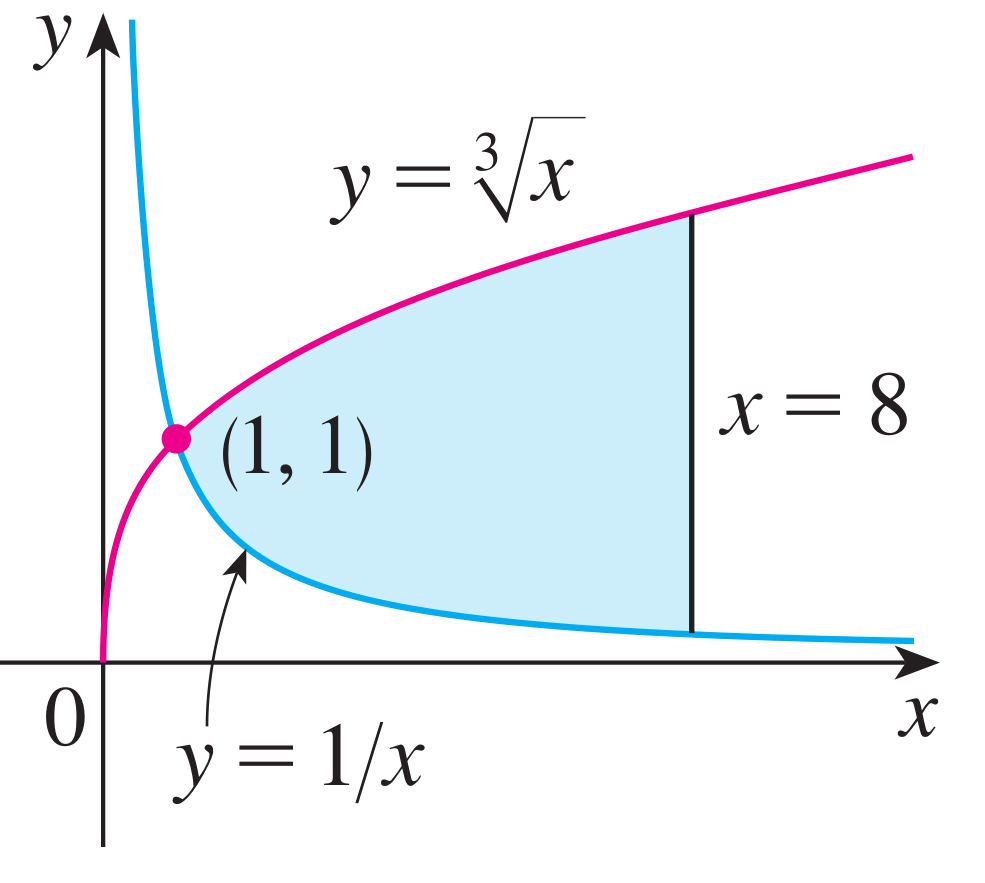
\includegraphics[scale=.2]{1.PNG}
			\vfill
			\item 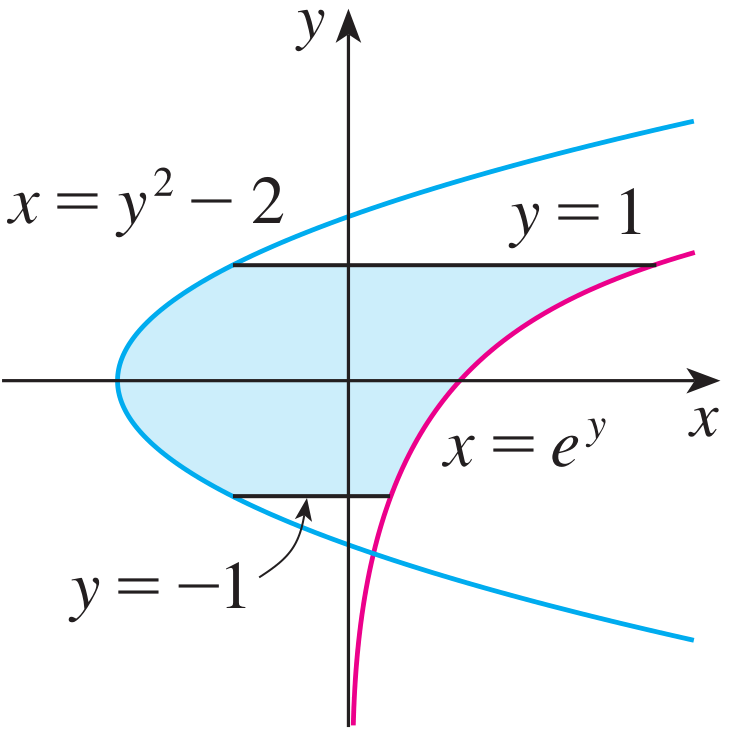
\includegraphics[scale=.25]{2.PNG}
		\end{enumerate}
		\vfill\null\columnbreak

		\item Sketch the region enclosed by the given curves and find its area.
		\begin{enumerate}
			\item $y = x^2$, $y = 4x-x^2$.
			\vfill
			\item $y = x^4$, $y = 2-|x|$.
			\vfill
			\item $x = 2y^2$, $x = 4+y^2$.
		\end{enumerate}
		\vfill
		\item Find the area between the top half of a circle of radius 1 and $y = \frac{3}{5}\sqrt{1-x^2}$.
		\vfill
	\end{enumerate}
\end{multicols*}

\end{document}